\documentclass[11pt,a4paper,titlepage, ngerman]{article}

\usepackage[utf8]{inputenc}	
\usepackage[T1]{fontenc}	
\usepackage{ngerman}			
\usepackage{lmodern}			
\usepackage{graphicx}			
\usepackage{url}				
\usepackage{siunitx}
\usepackage{amsmath}			
\usepackage{subcaption}
\usepackage{wrapfig}

\newcommand{\refeq}[1]{Gl. (\ref{eq:#1})}
\newcommand{\reffig}[1]{Fig. \ref{fig:#1}}
\newcommand{\reftab}[1]{Tab. \ref{tab:#1}}

\begin{document}

	\begin{titlepage}
		\centering
		{\scshape\LARGE Versuchsbericht zu \par}
		\vspace{1cm}
		{\scshape\huge E5 -- Magnetische Suszeptibilität\par}
		\vspace{2.5cm}
		{\LARGE Gruppe 10 Mi\par}
		\vspace{0.5cm}
		{\large Alex Oster (E-Mail: a\_oste16@uni--muenster.de) \par}
		{\large Jonathan Sigrist (E-Mail: j\_sigr01@uni--muenster.de) \par}
		\vfill
		durchgeführt am 15.11.2017\par
		betreut von\par
		{\large Phillip \textsc{Eickholt}}		
		\vfill	
		{\large \today\par}
	\end{titlepage}
		
	\tableofcontents
		
	\newpage
	
	\section{Kurzfassung}
		
		In diesem Bericht beschäftigen wir uns mit den magnetischen Eigenschaften von Stoffen.
		Dazu gehen wir insbesondere auf \glqq schwache\grqq{} Arten magnetischer Eigenschaften ein, welche im Alltag unscheinbar wirken, dennoch existieren.
		Um diese nachzuweisen, betrachten wir hier vier Versuche.
		Der Erste beschäftigt sich mit den magnetischen Eigenschaften von Wasser bzw. Manganchlorid, welche wir durch das Einschieben eines äußeren Magnetfeldes betrachten können.
		Um die Größenordnung der dabei entstehenden Auslenkungen zu bestimmen, führen wir eine Fermi-Abschätzung durch.
		
		Bei dem zweiten Versuch bestimmen wir mit Hilfe einer Magnetismuswaage die Volumensuszeptibilität bzw. die Magnetisierbarkeit von Aluminium, Graphit und Glas in einem äußeren Magnetfeld.
		
		Zuletzt betrachten wir, welchen Einfluss die Geometrie eines Stoffes (hier Aluminium), welcher sich in einem äußeren Magnetfeld befindet, auf seine magnetischen Eigenschaften hat.
		In Versuch 3 betrachten wir dazu das Fallen eines starken Magnets durch zwei Typen von Rohren und in Versuch 4 zwei Aluminiumplatten verschiedener Form bei Anlegen eines äußeren Magnetfeldes.		

	\section{Arten von Magnetismus}
				
		Alle Stoffe besitzen magnetische Eigenschaften, wobei die beim Anlegen eines äußeren Magnetfeldes auftretenden Effekte bei den meisten Stoffen verschwindend gering sind. Die Stärke dieser Effekte ist abhängig von dem Magnetismustypen des Stoffes\footnote{dieser steht in Abhängigkeit von der Temperatur, kann sich demnach ändern}. 
				
		Wir betrachten im Folgenden zwei Typen von Magnetismus, welche für die durchgeführten Versuche relevant sind: Dia- und Paramagnetismus. Hier gehen wir zuerst auf die makroskopische und dann auf die mikroskopische Betrachtung dieser Phänomene ein.
		
		\subsection{Diamagnetismus}
		
			Ist ein Stoff diamagnetisch, so bedeutet das, dass bei Anlegen eines äußeren Magnetfeldes eine kleine Magnetisierung des Stoffes entgegengesetzt zu Richtung dieses Feldes induziert wird.
			Dies bedeutet, dass Diamagnete in einem inhomogenen äußeren Magnetfeld aus Bereichen mit stärkerem Feld leicht abgestoßen werden. Ohne ein solches äußeres Magnetfeld verschwinden die diamagnetischen Eigenschaften des Stoffes.

			Aufgrund der Struktur von Materie führt der Spin jedes Eektrons unter Einfluss eines äußeren Magnetfeldes zu einem Ringstrom. 
			Dieser hat induktiv eine Magnetisierung entgegen diesem äußeren Feld zu Folge.
			Solche magnetischen Strommomente $\mu _\text{Strom}$ sind allgemein in Materie vorzutreffen.
				
		\subsection{Paramagnetismus}
			
			Paramagnetische Stoffe hingegen werden durch kleine Magnetisierung in Richtung des äußeren Magnetfeldes zu diesem gezogen, da sie hierbei eine Kraft in Richtung höherer Magnetfeldstärke erfahren. 
			Wie auch bei diamagnetischen Stoffen, verschwinden die paramagnetischen Eigenschaften, wenn das äußere Magnetfeld nicht weiter vorhanden ist.
			
			Das magnetische	Moment $\mu _\text{Spin}$ ergibt sich aus dem Spin- und Bahnmoment ungepaarter Elektronen.
			Im Gegensatz zu den diamagnetischen Stoffen sind die magnetischen Momente $\mu _\text{Spin}$ deutlich größer als die magnetischen Strommomente $\mu _\text{Strom}$, die Magnetisierung in Rightung des äußeren Feldes überwiegt also.
			Für vollständig gefüllte Atomschalen ist dieser Effekt nicht möglich, da hier keine freien Elektronen vorhanden sind.			
			
	\section{Versuch 1: Demonstrationsversuch} 
		
		Der erste Versuch war ein Demonstrationsversuch.
		Er wurde von unserem Betreuer durchgeführt und diente dazu, die Effekte der beiden schwachen Magnetisierungen zu verdeutlichen.
		Ziel war es, die durch ein äußeres Magnetfeld verursachte Auslenkung einer Flüssigkeit abzuschätzen.
		
		\subsection*{Methoden} 
		
		Es wurde ein Laser auf Wasser in einer dünnen Schale gerichtet.
		Die Reflexion des Lasers von der Wasseroberfläche war an der gegenüberliegenden Wand\footnote{Die Wand wird im Folgenden als Schirm bezeichnet.} zu sehen.
		Wir schieben einen starken Magneten unter der Schale her und betrachten die Reflexion am Schirm.
		In Abbildung \ref{fig:Fermi1} ist dies schematisch dargestellt.
		Der Laser ohne Magnet ist hier in rot zu sehen und mit Magnet in orange.
		Wir betrachten zur Berechnung der Auslenkung des Wassers $h$ die Änderung des Austrittswinkels, wie es in Abb. \ref{fig:Fermi2} genauer dargestellt ist.
		\begin{figure}[ht]
			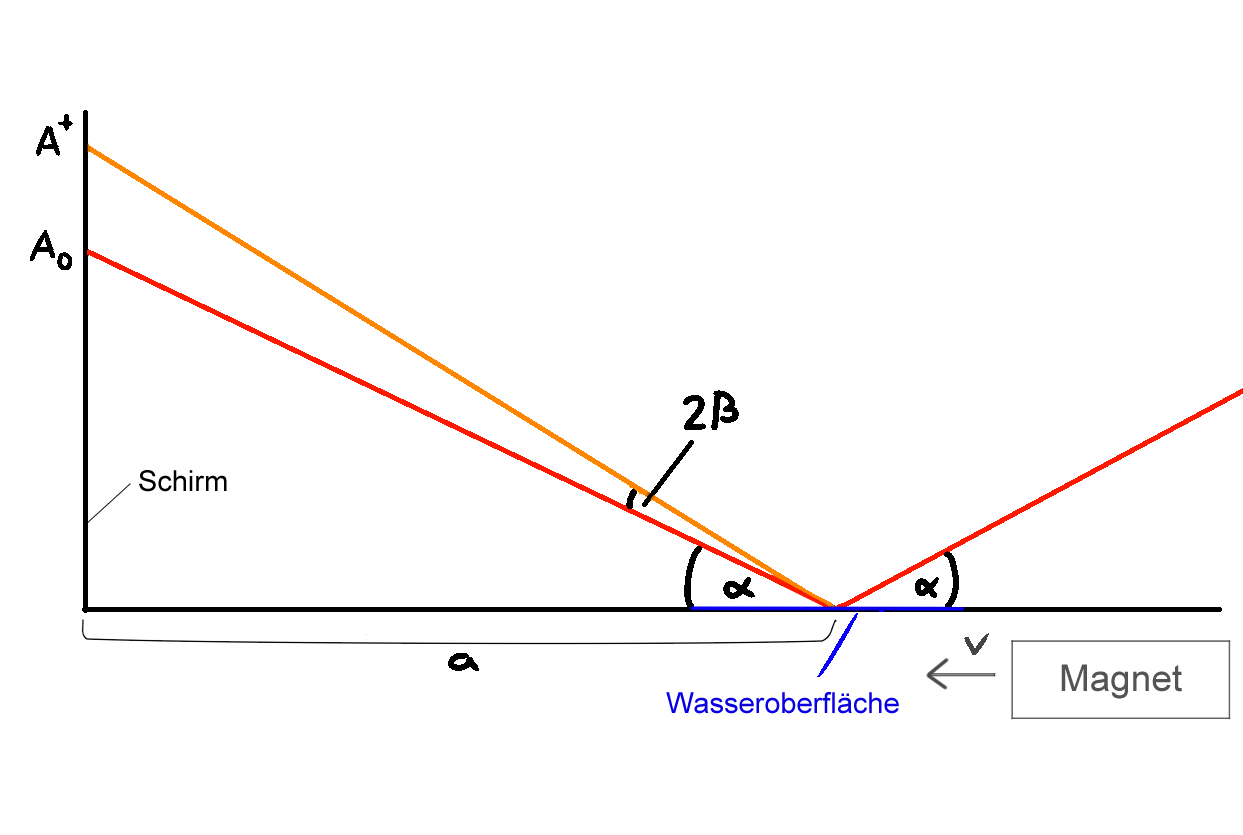
\includegraphics[width=\textwidth]{SkizzeFermi1.png}
			\caption{Aufbau des Demonstrationsversuchs.}
			\label{fig:Fermi1}
		\end{figure}
		\begin{figure}[ht]
			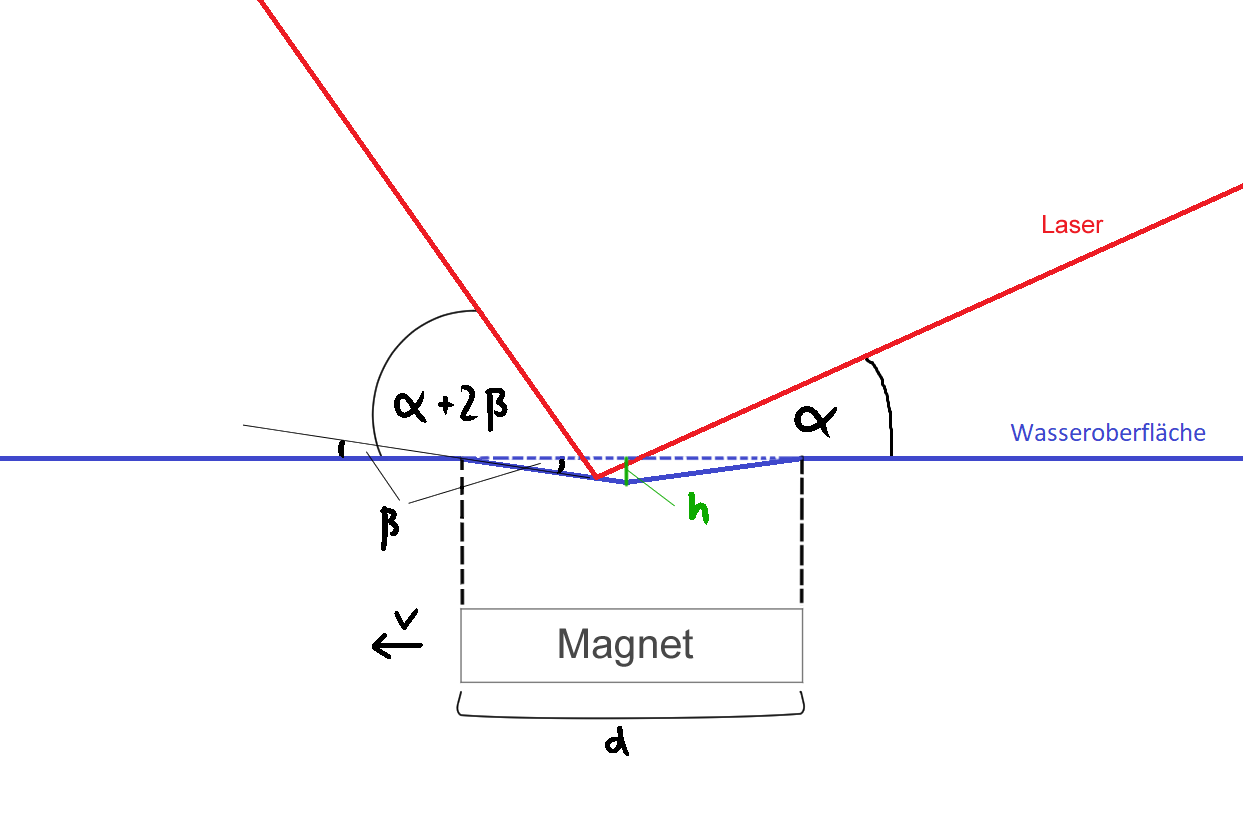
\includegraphics[width=\textwidth]{SkizzeFermi2.png}
			\caption{Genauere Betrachtung der Oberfläche.}
			\label{fig:Fermi2}
		\end{figure}
	
		Dazu betrachten wir folgende Gleichungen:
		
		Aus Abbildung \ref{fig:Fermi1} folgt
		\begin{align}
			\tan \alpha &= \frac{A_0}{a}
			\label{eq:schirm1}\\
			\tan (\alpha + 2 \beta) &= \frac{A^+}{a};\quad A^+ = A_0+\Delta A
			\label{eq:schirm2}
		\end{align}
		
		und aus Abb. \ref{fig:Fermi2} folgt
			\begin{align}
			\tan \beta = \frac{2 h}{d}.
			\label{eq:kruemmung}
		\end{align}
											
		Stellt man nun \refeq{kruemmung} nach der gesuchten Größe $h$ um und setzt geeignet \refeq{schirm1} und \refeq{schirm2} ein, so folgt:	
		\begin{align*}
			\tan \beta = \frac{2h}{d} \Leftrightarrow h &= \frac{d}{2} \tan \beta\\
			&= \frac{d}{2} \tan \left( \frac{1}{2}\arctan \left( \frac{A^+}{a}\right) - \frac{\alpha}{2}\right)\\
			&= \frac{d}{2} \tan \left( \frac{\arctan \left( \frac{A^+}{a}\right) - \arctan\left( \frac{A_0}{a}\right)}{2} \right)
		\end{align*}
				
		\subsection*{Fermi-Abschätzung}
				
			Um herauszufinden in welcher Größenordnung die Auslenkung des Wassers liegt, haben wir eine Fermi-Abschätzung durchgeführt.
			Dafür nehmen wir folgende Werte an:
			\begin{equation*}
				a = \SI{3,5}{\meter};\quad
				A_0 = \SI{1,2}{\meter};\quad
				\Delta A = \SI{3}{\centi\meter};\quad
				d = \SI{1}{\centi\meter}
			\end{equation*}
			Wir erhalten durch Einsetzen in die obige Gleichung ein Ergebnis von $h \approx \SI{19}{\micro\meter}$ für die Auslenkung des Wassers.
			In Abb. \ref{fig:zeitverlauf} ist die ungefähre Auslenkung in Abhängigkeit von der Magnetposition dargestellt. 
			Mit Abb. \ref{fig:Fermi2} kann man erkennen, dass das Wasser unter dem Magnetfeld eine Kuhle bilden muss, damit der Strahl erst weiter nach oben reflektiert wird.
			Das Wasser muss also diamagnetisch sein.
			
			Zudem haben wir den Versuch mit einem Manganchlorid-Hydrat anstelle von Wasser wiederholt und eine deutlich größere Auslenkung des Lasers wahrgenommen, diesmal jedoch zunächst in negative Richtung.
			Mit $\Delta A = \SI{0,7}{\meter}$ erhalten wir durch Fermi-Abschätzung eine Auslenkung von $h \approx \SI{420}{\micro\meter}$.
			Da sich der Laser zuerst nach unten bewegt hat, muss Manganchlorid-Hydrat Paramagnetisch sein.
			
			\begin{figure}[ht]
				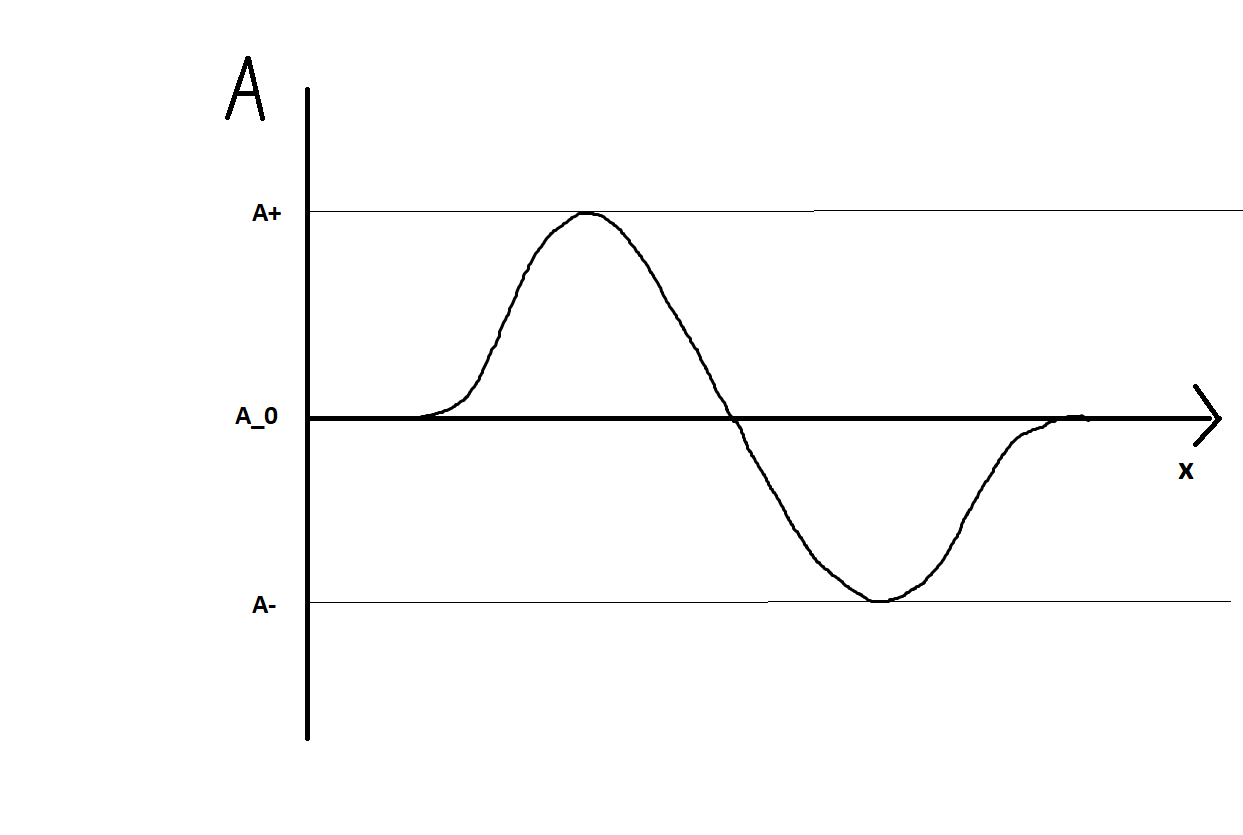
\includegraphics[width=\textwidth]{SkizzeZeitverlaufLichtpunktWasser.png}
				\caption{Verlauf des Lichtpunktes auf dem Schirm gegen die Position des Magneten.}
				\label{fig:zeitverlauf}
			\end{figure}

		\subsection*{Schlussfolgerung}
		
			Die von uns ermittelte Größenordnung der Auslenkung für Wasser wirkt realistisch, da es diamagnetisch ist, also nur sehr schwach auf äußere Magnetfelder reagiert.
			Die Betrachtung des Manganchlorids stellt seine paramagnetischen Eigenschaften deutlich in Kontrast zu den diamagnetischen des Wassers.
			Es reagiert sehr viel stärker und die Magnetisierung des Stoffes ist genau entgegengesetzt.
			Diese Kontraste entsprechen den Definitionen von Dia- und Paramagnetismus.
			
	\section{Versuch 2: Magnetismuswaage  und Volumensuszeptibilität}		
		
		In dem zweiten Versuch bestimmen wir mit Hilfe der Magnetismuswaage die Volumensuszeptibilität $\chi _V$ von Aluminium, pyrolitisches Graphit und Glas. Diese gibt an, wie stark sich ein Stoff magnetisieren lässt.		
		
		\subsection*{Methoden} 
		
			Die Magnetismuswaage, wie sie in Abb. \ref{fig:Magnetismuswaage} dargestellt ist, dient zur Messung der Gewichtsänderung eines Stoffes bei anliegendem äußerem Magnetfeld.
			Dieses stammt von einem starken Magneten, welcher mit einem Schwenkarm fest auf einer Höhe gehalten werden kann.
			Um eine möglichst genaue Messung durchzuführen soll der Abstand zwischen Stoffprobe und Magnet immer der gleiche sein.
			Um die Höhe des Magneten einzustellen, verwenden wir eine \SI{1}{mm} dicke Kunststoffplatte und legen sie zwischen Probe und Magneten, sodass der Abstand gerade dieser Dicke entspricht.
			\begin{figure}[ht]
				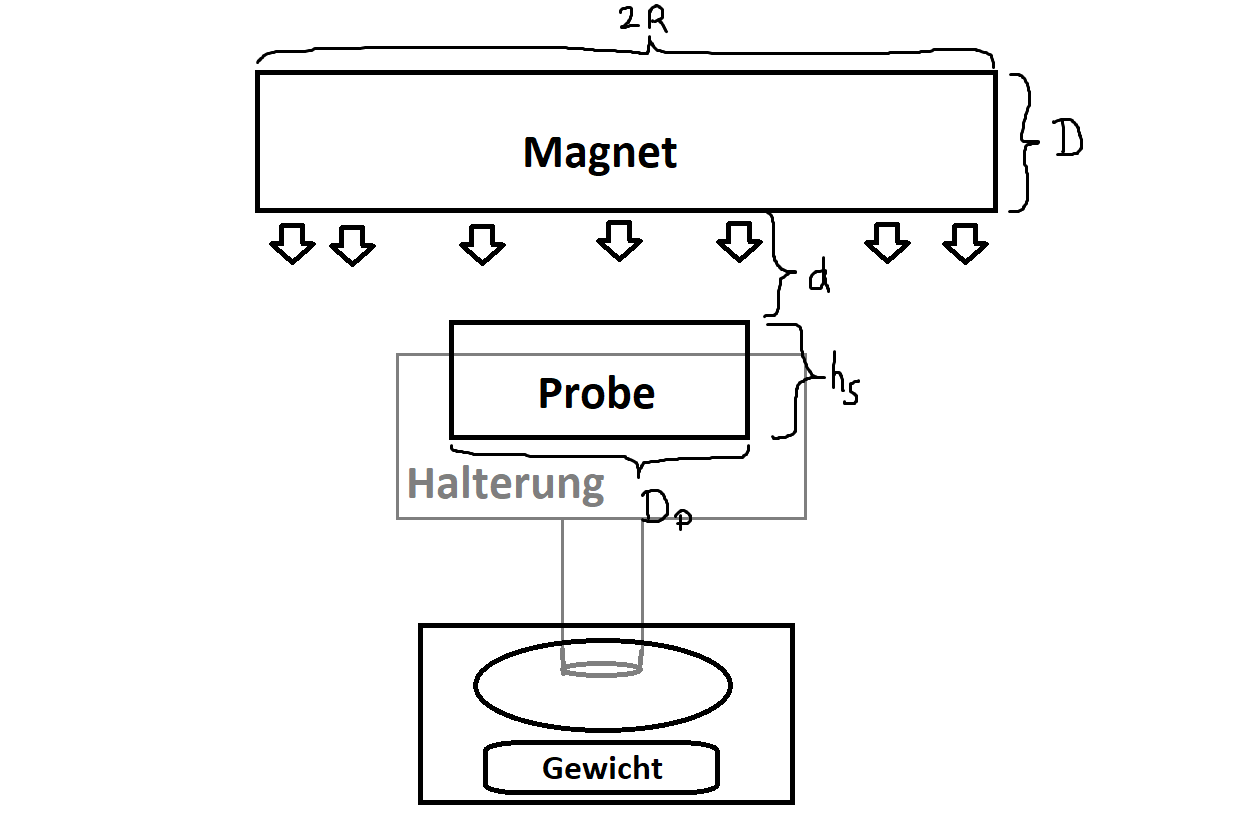
\includegraphics[width=\textwidth]{SkizzeMagnetwaage.png}
				\caption{Aufbau der Magnetismuswaage.}
				\label{fig:Magnetismuswaage}
			\end{figure}
						
			Damit der Magnet die einfache Messung des Gewichts der Stoffprobe nicht beeinflusst, wird er mit dem Schwenkkran zunächst wegbewegt.
			Für die Messung selber nullen wir zuerst das Gewicht unserer Stoffprobe und fahren dann den Magneten über die Probe und messen den Gewichtsunterschied.
			Dabei zeigt die digitale Waage Gewichtsänderungen von \SI{0,01}{g} an, was zu einer Unsicherheit von $u(m) = u(\Delta m) = \frac{\SI{0,01}{g}}{2\sqrt{3}}$ führt.
		
			Um nun aus dem Gewichtsunterschied die Volumensuszeptibilität $\chi _V$ zu erhalten, gehen wir auf folgende Gleichungen ein:
			\begin{equation*}
				\chi_V = \frac{2 \cdot \mu_0 \cdot \Delta m \cdot g}{V_S \cdot \frac{\partial\,B^2_z}{\partial\,z}},
			\end{equation*}
			wobei näherungsweise gilt
			\begin{equation*}
				\frac{\partial\,B^2_z}{\partial\,z} \approx \frac{B_z^2(d) - B_z^2(d+h_s)}{h_s}.
			\end{equation*}
			Hierbei ist $h_s$ die Höhe der Probe und $d$ der Abstand der Probe zum Magneten ($d = \SI{1}{\mm}$).\\
			Für das Magnetfeld gilt
			\begin{equation*}
			B(z) = \frac{B_r}{2}\left( \frac{D+z}{\sqrt{R^2 + (D+z)^2}} - \frac{z}{\sqrt{R^2 + z^2}}\right)
			\end{equation*}
			mit spezifisch $B_r = \SI{1,87+-0,1}{T}$, sowie Radius $R = \SI{30}{\milli\meter}$ und Dicke $D = \SI{15}{\milli\meter}$.
			
			Setzt man die Gleichungen ein, so folgt
			\begin{equation}
			\chi_V = \gamma \frac{\Delta m}{B_r^2}
			\label{eq:chi_V}
			\end{equation}
			mit den Konstanten
			\begin{align*}
			\gamma = \frac{8 \cdot \mu_0\cdot g \cdot h_S}{V_S \cdot \alpha},\quad
			\alpha = \left( B_z^{'}(d)\right)^2-\left( B_z^{'}(d+h_S)\right) ^2\\
			\text{und }B_z^{'}(z) = \frac{D+z}{\sqrt{R^2 + (D+z)^2}} - \frac{z}{\sqrt{R^2+z^2}}.
			\end{align*}
			
			Die Unsicherheit ist dann gegeben durch
			\begin{equation}
				u(\chi_V) = \gamma\sqrt{\left( \frac{u(\Delta m)}{B_z^2}\right) ^2+\left( \frac{\Delta m}{2B_z^3}u(B_r)\right) ^2}.
			\end{equation}
				
		\subsection*{Messung}
			
			In Tab.\ref{tab:Messergebnisse} sind die Ergebnisse dargestellt.
			Dabei wurden folgenden Werte für die Berechnung der Volumensuszeptibilität $\chi _V$  verwendet:
			\begin{align*}
				D = \SI{15}{\milli\meter}; \quad R = \SI{30}{\milli\meter}; \quad B_r = \SI{1,87}{T}; \quad u(B_r) = \SI{0,1}{T}\\
				d = \SI{1}{\milli\meter}; \quad r = \SI{20}{mm}; \quad V_s = h_s \cdot \pi r^2\\
				h_\text{Glass} = \SI{8}{mm}, \quad h_\text{Aluminium} = h_\text{Graphit} = \SI{5}{mm}.
			\end{align*}
			Die Massendifferenz in $\chi_V$ ist die Differenz von Masse der Halterung mit Probe und Masse der Halterung ohne Probe unter Einfluss des Magnetfeldes.
			
				\begin{table}[ht]
					\centering
					\begin{tabular}{l|S|S|S}
						\hline
						 & {Aluminium} & {pyr. Graphit} & {Glas} \\
						\hline
						$\chi _V$
						& \SI{13,79 +- 1,38}{\micro{}}
						& \SI{-634,49 +- 17,01}{\micro{}}
						& \SI{-11,60 +- 0,89}{\micro{}}\\
						\hline
					\end{tabular}
					\caption{Volumensuszeptibilität für die Proben.}
					\label{tab:Messergebnisse}
			\end{table}
					
		\subsection*{Schlussfolgerung}	
			
			Die von uns erhaltenen Wert für die Volumensuszeptibilitäten von Aluminium und Graphit korrelieren nicht signifikant mit den Literaturwerten.
			Zwar sind unsere Erwartungswerte in den selben Größenordnungen, die Literaturwerte liegen dennoch mehrere Unsicherheiten von diesen entfernt.
			Dadurch ist der Vertrauensgrad sehr gering.
			Lediglich der Wert für Graphit bestätigt den Literaturwert mit hohem Vertrauensgrad.
			
			Nach unserer Messung ist Aluminium paramagnetisch.
			Graphit ist diamagnetisch und die Volumensuszeptibilität ist bedeutend größer als die von Aluminium.
			Glas ist hingegen nur schwach diamagnetisch.
		
	\section{Versuch 3: Fallender Neodymmagnet}		
	
		Bei diesem Versuch lassen wir einen Neodymmagnet durch zwei Röhren aus Aluminium fallen. Eine der beiden Röhren besitzt einen Schlitz, der sich über die gesammte Länge zieht. Der Aufbau ist in Abb. \ref{fig:Neodymmagnet} dargestellt.
		\begin{figure}[ht]
			\centering
			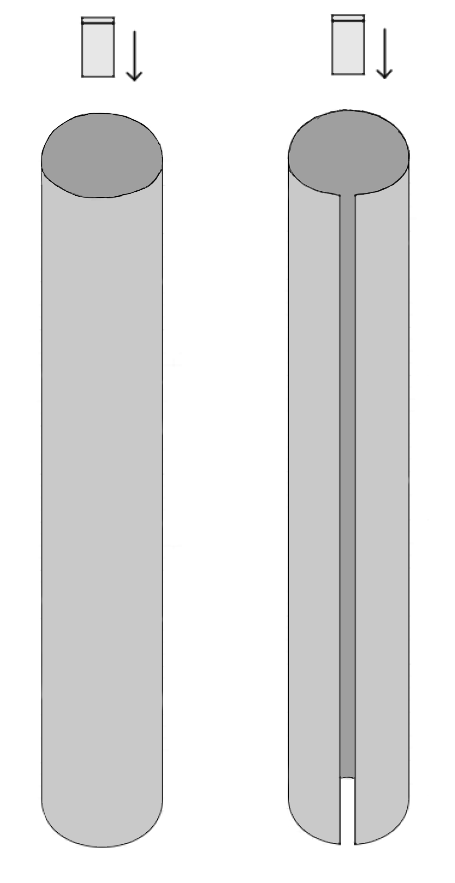
\includegraphics[width=0.4\textwidth]{Neodymmagnet.png}
			\caption{Darstellung der beiden Röhren mit und ohne Schlitz.} 
			\label{fig:Neodymmagnet}
		\end{figure}
		
		\subsection*{Beobachtung}
			
			Lässt man den Magneten durch die Röhre mit Schlitz fallen, so braucht er länger, als im freien Fall.
			In der vollständigen Röhre braucht der Magnet sogar noch länger.
			
		\subsection*{Schlussfolgerung}	
		
			Das bewegte B-Feld des Magneten induziert einen Kreisstrom in der Aluminiumröhre.
			Dieser erzeugt dann ein entgegengesetztes B-Feld, durch welches der Magnet abgebremst wird.
			Da der Kreisstrom von der Bewegungsgeschwindigkeit abhängt, gibt es eine kritische Geschwindigkeit, bei der die Lenz'sche Rücktreibungskraft gerade der Gravitationskraft entspricht.
			
			Für die Röhre mit Schlitz wird ebenfalls ein Strom induziert.
			Durch die Öffnung kann sich dieser jedoch nicht um die gesammte Röhre ausbreiten.
			Es bildet sich also kein die Röhre umschließender Kreisstrom und das Gegenfeld ist bedeutend schwächer.
			Die kritische Geschwindigkeit ist folglich höher und der Magnet fällt schneller.		
					
	\section{Versuch 4: Aluminium-Kamm und -Platte} 
	
		Eine Aluminiumplatte und ein -kamm sind an einer Aufhängung befestigt und können frei in einer Richtung schwingen.
		In Abb. \ref{fig:Aluplatte} sei dies schematisch dargestellt.
		Es sei weiterhin angemerkt, dass sowohl die Platte als auch der Kamm in Richtung der Bildfläche schwingen können.
		An beiden Objekten bewegen wir nun einen Magnetstab von verschiedenen Richtungen und Geschwindigkeiten entlang.
		\begin{figure}[ht]
			\centering
			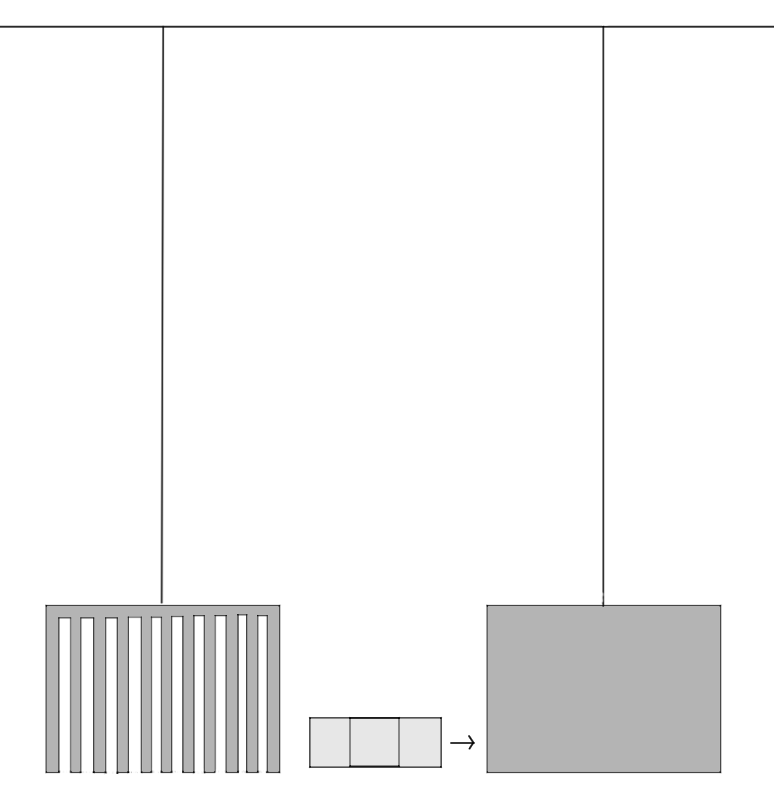
\includegraphics[width=0.6\textwidth]{Alu-Platte.png}
			\caption{Eine Aluminiumplatte und -Kamm an einer Aufhängung.} 
			\label{fig:Aluplatte}
		\end{figure}
		
		\subsection*{Beobachtung}
		
			Als wir den Magneten schnell und frontal auf die Aluminiumplatte bewegten, hat diese einen Ruck nach hinten gemacht.
			Berührte man die Platte, dann haftete sie an dem Magneten und bewegte sich mit diesem.
			Zog man den Magneten ruckartig von der Aluminiumplatte weg, hat die Platte ebenso einen Ruck nachgeahmt, diesmal stärker als beim heranführen.
			Nachdem der Magnet außer Reichweite war, pendelte die Platte unbeeinflusst nach.
			
			Bewegte man den Magneten jedoch langsam an die Aluminiumplatte heran, so wurde sie bei kleinen Abständen an den Magneten gezogen, entgegen der schnellen Bewegung. 
			Auch hier ließ sich die Platte bei dem Wegziehen des Magneten ein wenig mitziehen, jedoch nicht so weit, wie bei der schnellen Bewegung.
			
			Ein seitliches Heranführen des Magneten führte nur zu unkontrolliertem Wackeln der Platte und soll nicht weiter betrachtet werden.
			
			Für den Aluminiumkamm verliefen alle Beobachten analog, jedoch deutlich schwächer.
			
		\subsection*{Schlussfolgerung}	
			
			Aluminium ist paramagnetisch und wird von einem äußeren Magnetfeld angezogen.
			Zusätzlich wird durch die Änderung des Magnetfeldes ein Wirbelstrom in der Platte induziert.
			Führt man den Magneten nun schnell an die Platte heran, so überwiegt das Gegenfeld der Wirbelströme und die Platte stößt sich vom Magneten ab.
			Bei dem langsamen Annähern ist das Gegenfeld kleiner und die paramagnetischen Effekte ziehen die Platte zum Magneten.
			
			Bei dem Aluminiumkamm sind diese Effekte schwächer, da sich aufgrund seiner Geometrie keine großen Kreisströme bilden können und das daraus entstehende Magnetfeld somit schwächer ist.
		
\end{document} 